\section{Apparato sperimentale}\label{sec:apparato-sperimentale}
\subsection{Schema del circuito}\label{subsec:schema-circuito}

\begin{figure}[h]
  \centering
      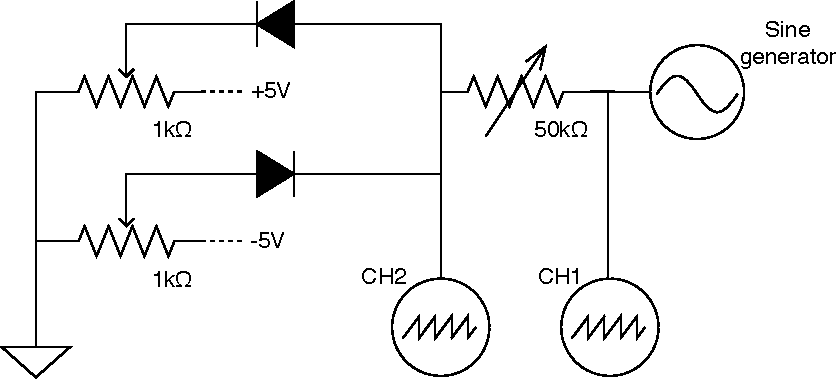
\includegraphics[width=10cm]{../assets/circuito.drawio.pdf}
      \caption{
        \emph{
          Schema del circuito tosatore.
        }
      }
    \label{fig:circuito}
\end{figure} %todo

Il circuito che abbiamo realizzato è schematizzato in figura \ref{fig:circuito}.
È strutturato come segue:
\begin{enumerate}
  \item%
  Due potenziometri da $1k\Omega$ sono collegati a terra e a $\pm 5V$, rispettivamente.
  \item%
  Due diodi al silicio (germanio) sono collegati al pin centrale dei potenziometri.
  \item%
  Un generatore di onda sinusoidale è collegato a una resistenza variabile da $50k\Omega$.
  \item%
  Un canale dell'oscilloscopio vede l'output \emph{pulito} del generatore di funzione.
  \item%
  Un canale dell'oscilloscopio è collegato in parallelo ai due diodi e all'altro capo della resistenza variabile da $50k\Omega$.
\end{enumerate}
Il circuito così realizzato permette di regolare l'ampiezza dell'onda tosata e la curvatura
della porzione tosata.
Per fare ciò, bisogna agire rispettivamente sui due potenziometri da 1k$\Omega$
e sul potenziometro da 50k$\Omega$.

\subsection{Materiale e strumenti usati}\label{subsec:materiali}
Segue una lista del materiale e degli strumenti usati durante la prova:
\begin{itemize}
  \item%
  Oscilloscopio analogico, modello: \emph{GW Instek GOS-652}.
  \item%
  Multimetro digitale, modello: \emph{ISO-TECH IDM 105}.
  \item%
  Generatore di tensione, modello: \emph{Aim-TTi EB2025T}.
  \item%
  Generatore di onda sinusoidale, modello: \emph{GFG-8017G}.
  \item%
  Sonda per oscilloscopio.
  \item%
  Connettori vari (connettori a banana, cavi per la scheda millefori).
  \item%
  2 diodi al silicio
  \item%
  2 diodi al germanio
  \item
  2 potenziometri da $1k\Omega$.
  \item
  Potenziometro da $50k\Omega$.
\end{itemize}
